\vspace{-3mm}
%\section{Letter}
\paragraph{Introduction.}
%\label{sxn:body}
%\vspace{-1mm}

Recent work by Martin and Mahoney~\cite{MM18_TR,MM19_HTSR_ICML} has developed a new Theory of Implicit Heavy-Tailed Self-Regularization (HT-SR) for Deep Neural Networks (DNNs). 
Among other things, this theory provides a Universal empirical metric that characterizes the amount of \emph{Implicit Self-Regularization}---and, accordingly, the generalization capacity---for a wide range of publicly-available, best-in-class, pre-trained DNNs, including AlexNet, VGG, ResNet, \charles{including over 100 pre-trained models.}

In more detail, they study the Empirical Spectral Density (ESD), $\rho(\lambda)$, of individual layer weight matrices, $\mathbf{W}$, as well as of convolutional feature maps, through the lens of Random Matrix Theory (RMT); and they observe that the individual layer ESDs almost always follow a \red{(truncated)} power law (PL) distribution
\begin{equation}
\rho(\lambda)\sim\lambda^{-\alpha},\;\;\lambda\le\lambda_{max},
\label{eqn:eigenval_pl}
\end{equation}
where $\rho(\lambda)$ is the density of the eigenvalues $\lambda$ of the normalized layer correlation matrix 
\begin{equation}
 \mathbf{X} = \frac{1}{N}\mathbf{W}^{T}\mathbf{W},
\end{equation}
\red{and $\lambda_{max}$ is the maximum eigenvalue observed.}
The PL exponents nearly all lie within a universal range $\alpha\in[2,5]$, in nearly every pre-trained production-quality architecture considered.
See Figure~\ref{fig:alphas}.

\begin{figure}[H]
   \centering
   \subfigure[Power law exponents $\alpha$]{
     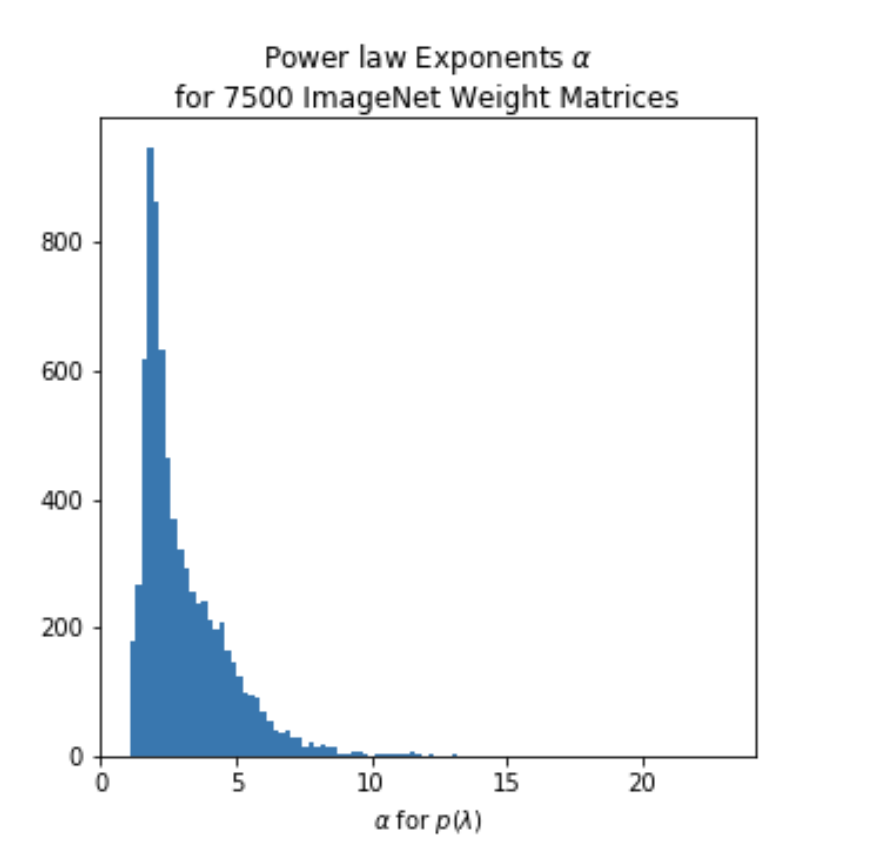
\includegraphics[scale=0.25]{img/power-law-histogram.png} 
     \label{fig:power-law-histogram}
   }
   \quad
   \subfigure[Average ${\alpha}$ vs Top5 error]{
      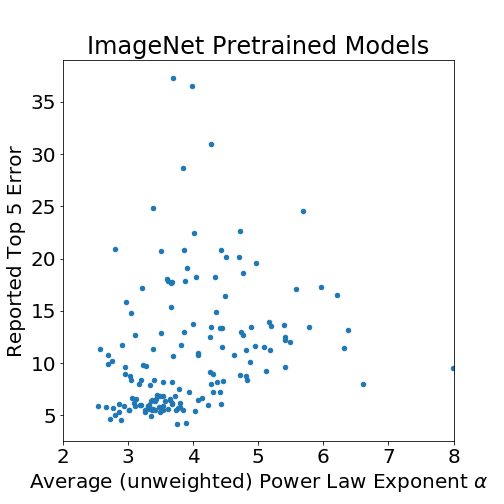
\includegraphics[scale=0.20]{img/Top5AvgAlpha.png}
      \label{fig:alphaTop5}
   }
   \caption{Histogram of PL exponents, and scatter plot of average ${\alpha}$ vs Top5 error, for nearly $10,000$ layer weight matrices (and 2D feature maps) from pre-trained DNNs, trained on ImageNet.
   \charles{Isn't this described in the text?}
   }
   \label{fig:alphas}
\end{figure}

These observations hold across nearly $10,000$ layer weight matrices (and 2D feature maps), drawn from over $50$ different, large-scale pre-trained DNNs, ranging over $15$ different architectures.
This includes DNNs pre-trained for computer vision (CV) tasks on ImageNet, as well as DNNs pre-trained for several different natural language processing (NLP) tasks.
Moreover, smaller values of $\alpha$ correlate well with better generalization accuracies, with $\alpha$ approaching a \emph{universal value}, $\alpha\rightarrow 2$, at the lower limit of the Moderately Heavy Tailed (or Fat Tailed) RMT Universality class~\cite{MM18_TR,MM19_HTSR_ICML} .  

In Statistical Physics, Universality of PL exponents is very special, and it suggests the presence of a deeper, underlying, \emph{Universal mechanism} driving the system dynamics~\cite{SornetteBook,BouchaudPotters03}.
It is this \emph{Heavy Tailed Mechanistic Universality} (HT-MU), as well call it, that originally motivated our study.  

HT-MU applies to the analysis of complicated systems, including many physical systems~\cite{SornetteBook}, traditional NNs~\cite{EB01_BOOK,nishimori01}, and even models of the dynamics of actual spiking neurons~\cite{XXX-SOME-NEURAL-SPIKE-PAPER}.
\michael{CHARELS: What is best ref here.} \charles{There are dozens, dating back decades:  A good, semi-recent Phys Rev ref is:  Friedman, N. et al. Universal critical dynamics in high resolution neuronal avalanche data. Physical Review Letters 108, 208102 (2012). }
Indeed, the dynamics of learning in DNNs, and perhaps real neurons as well, seems to resemble a system near a phase transition, e.g., the phase boundary of spin glass, a system displaying Self Organized Criticality (SOC), or a Jamming transition~\cite{GSdx18_TR,SGd18_TR}. 
Of course, we can not say which mechanism, if any, is at play. 
Instead, we use the machinery of  HT-RMT as a stand-in for a generative model of the weight matrices in DNNs, and we use this to catalog and model the HT behavior of DNNs.%

Based on these ideas, we develop here a Universal capacity control metric, $\hat{\alpha}$.
This metric is a weighted average of the layer PL exponents, $\alpha_{l}$, of the DNN layer weight matrices,
\begin{equation}
\hat{\alpha}=\sum_{l\in L}\alpha_{l}\log\lambda_{l}^{max}  ,
\label{eqn:alpha_hat_specific}
\end{equation}
where $L$ indexes layers, and 
%where 
$\lambda_{l}^{max}$ is the maximum eigenvalue (i.e., Spectral norm) of layer correlation matrices~$\mathbf{W}_{l}$. 

\paragraph{Approach.} 
Our approach and intent differ from other theoretical studies in the DNN literature, although we can relate our results back to known results.
Most recently, e.g., Liao et al.~\cite{LMBx18_TR} used an appropriately-scaled, data-dependent Product Norm capacity control metric to bound worst-case generalization error for several small (not production-quality, but still interesting) DNN models, and they showed that the bounds are remarkably tight.
There is, in fact, a large body of work on norm-based capacity control metrics, both recent~\cite{LMBx18_TR, SHNx17_TR,PLMx18_TR} and~\cite{NTS14_TR,NTS15,NBMS17_TR,BFT17_TR,YM17_TR,KKB17_TR,NBS17_TR,AGNZ18_TR,ACH18_TR,ZF18_TR}, as well as much older~\cite{Bar97,MN09_TR}. 
These studies seek \emph{worst-case} complexity bounds, motivated in some cases to reconcile discrepancies with more traditional statistical learning theory, and they apply (when applied at all) to quite small NNs.

This approach contrasts with that of Martin and Mahoney~\cite{MM18_TR,MM19_HTSR_ICML}, who looked at empirical properties of a wide range of state-of-the-art models, and from this developed a metric that provides \emph{a posteriori} characterization of implicit regularization for typical-case DNNs.  
Thus, instead of using statistical learning theory principles to propose a metric that provides worst-case \emph{a priori} bounds, we seek here an \emph{average-case} or \emph{typical case} (where ``typical'' is for current state-of-the-art publicly-available pre-trained DNN models) complexity metric, viable in production settings as a guide to the development of better DNNs at scale.

\paragraph{Theory.} 
Let us write the Energy Landscape (or optimization function) for a typical DNN with $L$ layers, with activation functions $h_{l}(\cdot)$, and with weight matrices and 
biases $\mathbf{W}_{l}$ and $\mathbf{b}_{l}$, as follows: \charles{Can we get rid of this extra space ?}
\begin{equation}
E=h_{L}(\mathbf{W}_{L}\times h_{L-1}(\mathbf{W}_{L-1}\times(\cdots)+\mathbf{b}_{L-1})+\mathbf{b}_{L})  .
\label{eqn:dnn_energy}
\end{equation}

Typically, this model would be trained on some labeled data $\{d_{i},y_{i}\}\in\mathcal{D}$, using Backprop~\cite{LBOM12_tricks}, by minimizing the loss $\mathcal{L}=\sum_{i\in\mathcal{D}}[E(d_{i})-y_{i}]$.

For simplicity, we do not indicate the structural details of the layers (e.g., Dense or not, Convolutions or not, Residual/Skip Connections, etc.), nor do we consider the details of the optimizer or the training process.

Each layer is defined by one or more layer 2D weight matrices $\mathbf{W}_{l}$, and/or the 2D feature maps $\mathbf{W}_{l,i}$ extracted directly from 2D Convolutional (Conv2D) layers.
(We have not yet analyzed LSTM or other complex Layers.)   A typical modern DNN may have anywhere between 5 and 5000 2D layer matrices / feature maps.

We can relate our universality metric to the more traditional, data dependent,  Product Norm capacity metrics $\mathcal{C}$, defined as
\begin{equation}
\mathcal{C}\sim\Vert\mathbf{W}_{1}\Vert\times\Vert\mathbf{W}_{2}\Vert\cdots\Vert\mathbf{W}_{L}\Vert   .
\end{equation}
Using a standard trick from field theory, we consider the log Product Norm, which takes the form of an average log norm
\begin{eqnarray*}
\log\mathcal{C} &\sim& \log\bigg[\Vert\mathbf{W}_{1}\Vert\times\Vert\mathbf{W}_{2}\Vert\cdots\Vert\mathbf{W}_{L}\Vert\bigg]  \\
                &\sim& \bigg[\log\Vert\mathbf{W}_{1}\Vert+\log\Vert\mathbf{W}_{2}\Vert\cdots\log\Vert\mathbf{W}_{L}\Vert\bigg]  \\
                &\sim&  \langle\log\Vert\mathbf{W}\Vert\rangle=\dfrac{1}{N_{L}}\sum_{l}\log\Vert\mathbf{W}_{l}\Vert   .
\end{eqnarray*}

\charles{Notice that our capacity metric $\hat{\alpha}$ depends 2 parameters, the PL exponent $\alpha$, a measure of matrix sparsity, and nd the maximum eigenvalue $\lambda_{max}$, which
corrects for the matrix scale. Other capacity metrics either consider just the sparsity with a rank (i.e the Stable Rank), or the scale with a  matrix norm, like the Spectral or the Frobenius norm.}

When $\Vert\mathbf{W}\Vert$ is the Spectral norm, $\Vert\mathbf{W}\Vert_{2}\sim\lambda_{max}$, then our $\hat{\alpha}$ of Eqn.~(\ref{eqn:alpha_hat_specific}) is a weighted average of the log Spectral norms, where the weights are power law exponents $\alpha$. 
In this sense, our universal metric $\hat{\alpha}$ behaves like an \emph{average-case} version of what is a worst-case bound, but it is more suitable for applying to large, production-level DNNs.
 
When $\Vert\mathbf{W}\Vert$ is the Frobenius norm, $\Vert\mathbf{W}\Vert^{2}_{F}$, we can use results of HT RMT to interpret the PL exponents $\alpha$ as a type of Soft or Stable Rank. 
Specifically, when $\alpha$ is very small, we can relate $\alpha$ to the more familiar Stable Rank $\mathcal{R}^{log}_{s}$, expressed in log-units (and up to the $\frac{1}{N}$ scaling):
\begin{equation}
\mathcal{R}^{log}_{s}:=\dfrac{\log\Vert\mathbf{W}\Vert^{2}_{F}}{\log\lambda^{max}}  \approx \alpha  .
\end{equation}
Using this, one could implement our capacity metric as a regularizer to improve DNN training by implementing a Stable Rank regularizer (similar to how Spectral norm regularization is implemented~\cite{XXX-XXX-WHAT-IS-BEST-REF}.
\michael{MICHAEL TO DO: fill in best ref for there.}


\paragraph{Methodology.} 
To evaluate our metric, we introduce a new methodology to analyze the performance of large-scale pre-trained DNNs, including the VGG and ResNet series of models, as well nearly 200 other widely available models, and we study how capacity metrics correlate with the reported test accuracies.
 
This approach offers several advantages over common practice in the area, most notably the following.
\begin{itemize}
\item 
We do not need access to the original ImageNet data, just the pre-trained models (i.e., as distributed with PyTorch, on github, and/or from the ModelZoo).
\item
We do not need to engage in expensive training/retraining, architecture adjustment, hyperparameter tuning, etc.
\item 
Our results are easily reproducible.
To make things more reproducible, we provide a python command tool, \texttt{WeightWatcher}~\cite{weightwatcher_package_justURL}, that works with both PyTorch (v1) and Keras (v2) models, and that computes a wide range of average log capacity metrics.
\end{itemize}
 
We have applied our Universal capacity control metric $\hat{\alpha}$ to a wide range of large-scale pre-trained production-level DNNs.
%Notice that, 
For Linear DNN layers, we can simply replace the log Norm with our metric, whereas for Conv2D Layers, we can associate the ``Norm'' of the 4-index Tensor $\mathbf{W}_{l}$ to the sum of the $n_{l}=c\times d$ terms for each feature map, as follows:

\begin{eqnarray*}
\text{Linear Layer:} & & \log\Vert\mathbf{W}_{l}\Vert
%\quad 
\rightarrow 
%\quad 
\alpha_{l}\log\lambda_{l}^{max}  \\
\text{Conv2D Layer:} & & \log\Vert\mathbf{W}_{l}\Vert
%\quad 
\rightarrow 
%\quad 
\sum_{i=1}^{n_{l}}\alpha_{l,i} \log\lambda_{l,i}^{max} .
\end{eqnarray*}

\paragraph{Results.} 
Our Universal metric correlates very well with the reported average test accuracies across many series of pre-trained DNNs.
See Figures~\ref{fig:bothmodels} and~\ref{fig:alphahats}.

\michael{CHARLES: make a short paragraph of this; need details on figs in captions or text---put in a draft, and then I'll make a pass.}
\charles{
We present 2 complex examples of pretrained models with similar architectures of differing depths.  Figure~\ref{fig:vgg_alphahat} presents the VGG series of networks (VGG11, 13, 16, and 19, with an without Batch Normalization (BN), as available in PyTorch), and a large set of ResNet architectures.  Figure~\ref{fig:resnet_alphahat} presents results for several ResNet models,
ranging from ResNet10 to ResNet152 (available here).  We generate the $\hat{\alpha}$ metric using the weightwatcher tool, (hopefully) making these results trivial to reproduce.
  Notice, we do not have access to the  (ImageNet) test data, and compare $\hat{\alpha}$ to reported Top1 test errors.  Amazingly, our simple $\hat{\alpha}$ metric correlates very well with the reported Top1 test errors. 
  }
  
\begin{figure}[H]
   \centering
   \subfigure[$\hat{\alpha}$ for VGG series]{
      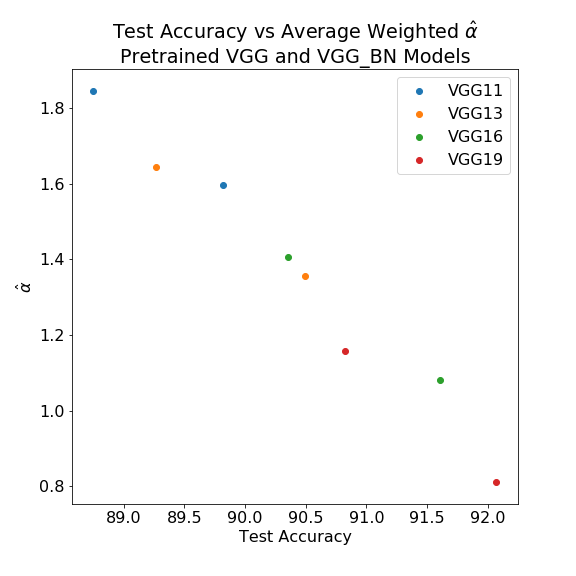
\includegraphics[scale=0.14]{img/vgg-w_alphas.png}
      \label{fig:vgg_alphahat}
   }
   \quad
   \subfigure[$\hat{\alpha}$ for ResNet series]{
      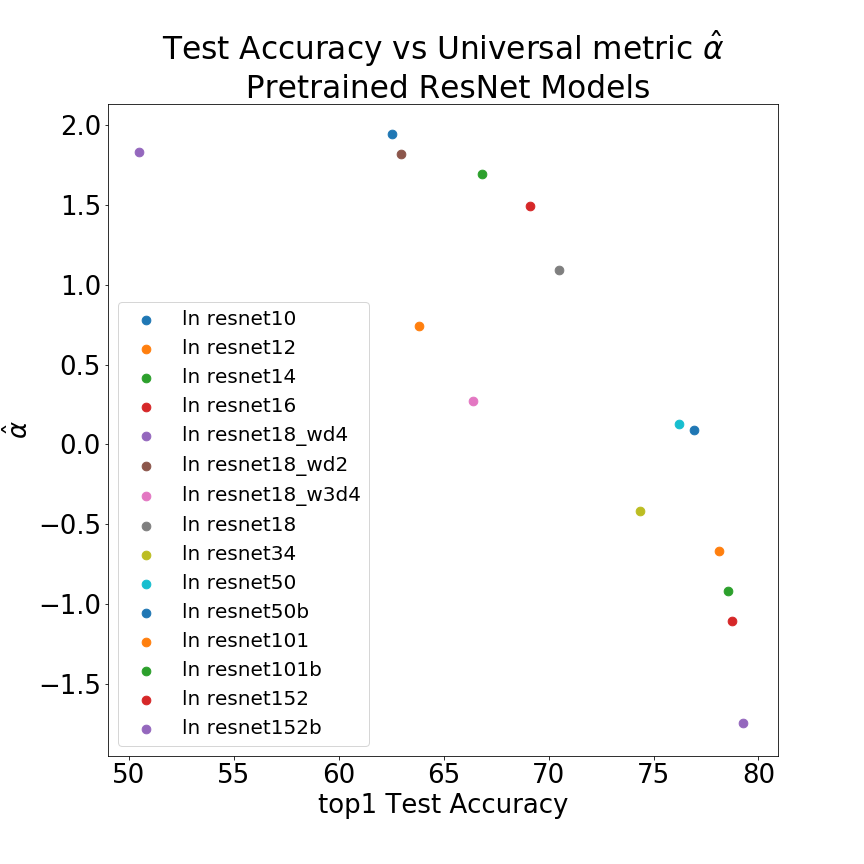
\includegraphics[scale=0.12]{img/ResNet-w_alphas.png}
      \label{fig:resnet_alphahat}
   }
   \caption{Top 1 Test Accuracy versus the Universal, weighted average PL exponent $\hat{\alpha}$ for pre-trained VGG and ResNet Architectures and DNNs.}
   \label{fig:bothmodels}
\end{figure}

\begin{figure}[H]
   \centering
    \subfigure[  $\hat{\alpha}$ vs Top1 error]{
      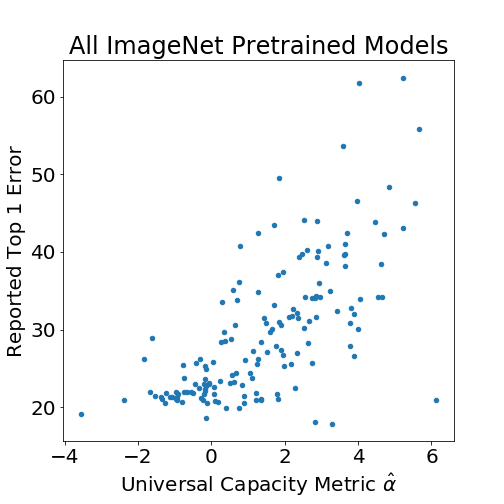
\includegraphics[scale=0.20]{img/Top1AlphaHat.png}
      \label{fig:alphahatTop1}
   }
   \caption{%
    Caption: we have room for 1 more 
    \michael{CHARELS: do we want another subfigure here, maybe scatter plot of some NLP models.}\charles{we do not have NLP data across architectures...still thinking about this}
   }
   \label{fig:alphahats}
\end{figure}


Our empirical results are, to our knowledge, the first time such theoretical capacity 
metrics have been reported to predict (trends in) the test accuracy for any series of DNNs, let alone for \emph{pre-trained production-level} DNNs.
In particular, this illustrates the usefulness of these norm-based metrics beyond smaller models such as MNIST, CIFAR10, and CIFAR100. 
Our  results can be reproduced with the \texttt{WeightWatcher} package~\cite{weightwatcher_package_justURL}; 
%\footnote{\url{https://pypi.org/project/WeightWatcher/}};
and our
results suggest that our ``practical theory'' methodology is fruitful more generally for engineering good algorithms for realistic large-scale DNNs.

\paragraph{Comparison with other metrics.}
Our Universality metric $\hat{\alpha}$ is related to other, more familiar capacity metrics such as the Spectral Norm, the Frobenius $(L2)$ Norm, and robust measures of matrix rank such as the Stable Rank.
This suggests an obvious question: 
Does the $\hat{\alpha}$ metric ``work'' simply because DNN models have explicit regularization (i.e., with an $(L2)$ or Spectral Norm constraint)?
More generally, is the $\hat{\alpha}$ metric just a variation of these more familiar \emph{worst case} bounds?  
\michael{MICHAEL TO DO: we seem to be convolving norms versus exponents with worst-case versus typical-case issues---I'll fix in light of recent discussion.}

The short answer is that we believe that HTMU is a new, more fundamental relation. 
It complements other metrics, but it works more generally on actual DNNs when other norm-based theoretical metrics inspired by worst-case bounds fail. 
In particular, we can identify counter examples, most notably in compressed DNN models~\cite{XXX-XXX-WHAT-IS-REF}\michael{MICHAEL TO DO: Fill in ref for compressed DNN models here}, where the average Frobenius $(L2)$ Norm increases with decreasing test error, but where the average $\alpha$ decreases, as expected.  


%For example, 
To illustrate this, we consider average metrics measured on ResNet20, trained on CIFAR10, before and after applying the Group Regularization technique, 
as implemented in the \emph{distiller} package~\cite{XXX-ADDCITE}. 
\michael{MICHAEL TO DO: Fill in reference for distiller here.}
\michael{MICHAEL TO DO: why is that in emph rather than texttt.}
See Figure~\ref{fig:resnet204D5L}.
\michael{CHARLES: More details here.}
%We compare the pre-trained baseline ($4D\_regularized\_5Lremoved$), with the pre-trained fine-tuned version ($4D\_regularized\_5Lremoved_finetuned$).    
Notice that the reported baseline test accuracies ($Top1=91.450$ and $Top5=99.750$) 
are better than the reported fine-tuned test accuracies ($Top1=91.020$ and $Top5=99.670$), so traditional theory suggests that the baseline Spectral Norm
($\lambda_{max}\sim\Vert\mathbf{W}\Vert_{2}$) should be \emph{smaller} than those of the layers in the fine-tuned model.
\michael{CHARELS: Frob norm not shown?  If yes, we can jsut say ``(not shown)'' but I want to check before adding that.}
\charles{YES}.
Based on previous empirical results, we may also expect the baseline Frobenius norm to be smaller than the fine tuned. 
%We observe the reverse for both.
In both cases, we observe the opposite.

\begin{figure}[H]
   \centering
   \subfigure[$\lambda_{max}$ for ResNet20 layers]{
      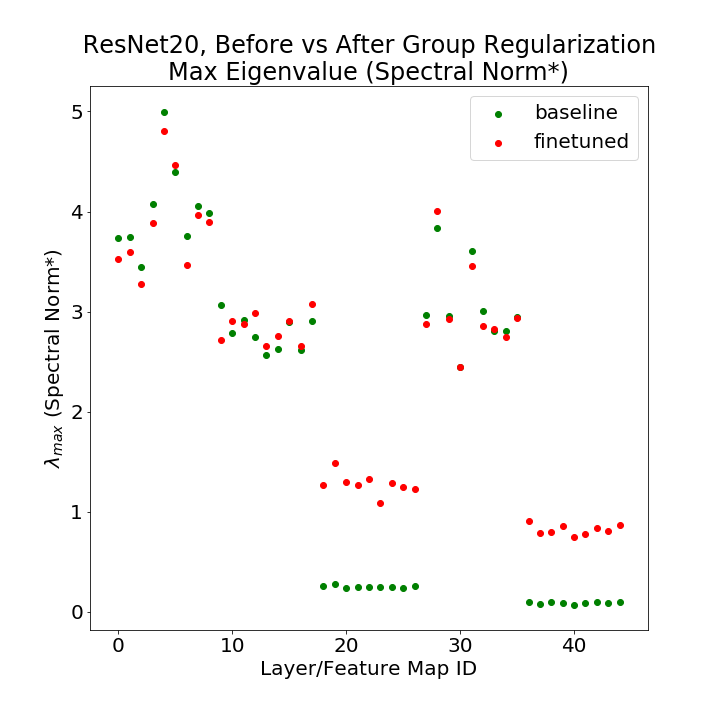
\includegraphics[scale=0.14]{img/resnet4d_maxev.png}
      \label{fig:resnet204Dalpha}
   }
   \quad
   \subfigure[$\alpha$ for ResNet20 layers]{
      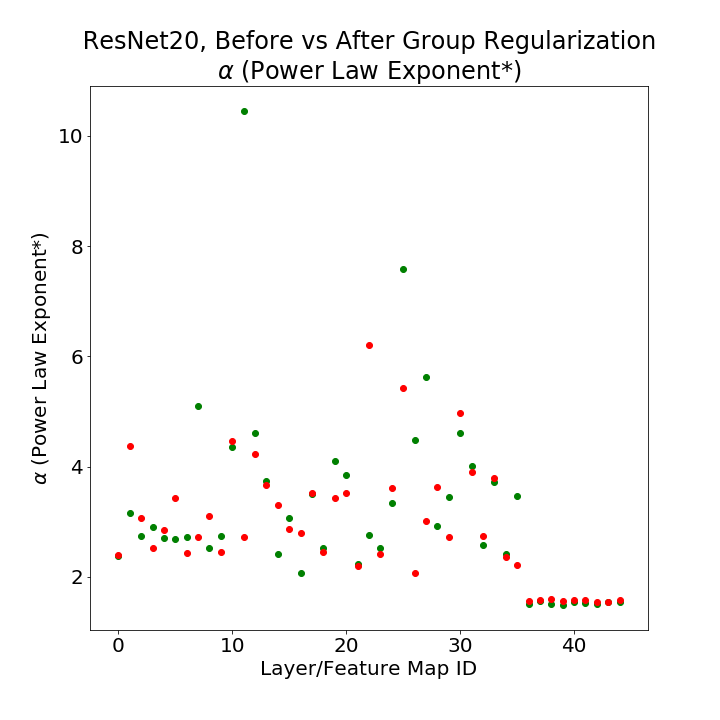
\includegraphics[scale=0.14]{img/resnet4d_alphas.png}
      \label{fig:resnet204Dmaxev}
   }
   \caption{
     ResNet20 with Group Regularization, comparison of layer $\mathbf{W}$ maximum eigenvalue ($\lambda_{max}$, or Spectral Norm *with $1/N$ normalization) and 
     Power Law exponent $\alpha$ pre-trained baseline and fine-tuned models.
     \michael{CHARLES: better explanation.}
           }
   \label{fig:resnet204D5L}
\end{figure}

\michael{CHARLES: Add a draft of that description; then I'll make a pass and make it a separate paragraph or combine with above par and below par.}
DESCRIBE THESE 2 FIGURES


For the $4D\_regularized$ models, the \emph{distiller} Group Regularization technique has the unusual effect of increasing the norms of the $\mathbf{W}$ feature maps for at least 2 of the Conv2D layers.
\michael{MICHAEL TO DO: name $4D\_regularized$ not introduced yet.}
We suspect this effect arises because the Group Regularization  concentrates Frobenius mass from the 5 removed Conv2D layers into these remaining Conv2D layers.

Notice while the matrix norms behave atyically, the layers $\alpha$ do not systematically differ between the baseline and fine-tuned models.
Also (not shown), the average (unweighted) baseline $\alpha$ is indeed smaller than the fine-tuned average
\michael{CHARLES: what is significance of that last comment.}\charles{--as predicted by our theory of HT-SR}

\paragraph{Discussion.}

We have presented an \emph{unsupervised} capacity control metric which predicts trends in test accuracies of a large-scale pre-trained DNN---without even peeking at the training data or the test data. 
This complexity metic, $\hat{\alpha}$ of Eqn.~(\ref{eqn:alpha_hat_specific}), is a weighted average of the PL exponents $\alpha$ for each layer weight matrix, where $\alpha$ is defined in the recent HT-SR Theory~\cite{MM18_TR,MM19_HTSR_ICML}, and where the weights are the largest eigenvalue $\lambda^{max}$ of the correlation matrix $\mathbf{X}$.  
%
We examine several commonly-available, pre-trained, production-quality DNNs, by plotting $\hat{\alpha}$ versus the reported test accuracies.
This covers classes of DNN architectures including the VGG models, ResNet, DenseNet, etc. 
In nearly every class, and except for only a few counterexamples, smaller $\hat{\alpha}$ corresponds to better average test accuracies, thereby providing a strong predictor of model quality for large-scale state-of-the-art DNN models.

It is worth emphasizing that we are taking a very non-standard approach (at least for the DNN and ML communities).
We did not train/retrain lots and lots of (typically rather small) models, analyzing training/test curves, trying to glean from them bits of insight that might then extrapolate to much-larger more realistic models.
Instead, we take advantage of the fact that there already exist many (typically rather large) publicly-available pre-trained models, and we analyze the properties of these models.
That is, we viewed these publicly-available pre-trained models as artifacts of the world that achieve state-of-the-art performance in CV, NLP, and related applications; and we attempted to understand why.
To do this, we extracted data-dependent metrics to predict generalization performance on production-quality models.
Given well-known challenges associated with training, and given our results here as well as other recent results~\cite{MM18_TR,MM19_HTSR_ICML},
we suggest that this methodology be applied more generally.

In theoretical physics, many researchers study neural networks using spin glass models, such as the traditional Gardner analysis~\cite{GD89,EB01_BOOK} and more recent work~\cite{PSG17_TR,PSG18_TR}.
Most notably, however, Choromanska et. al. have suggested that the energy landscape of DNNs should resemble the zero-temperature energy landscape of a p-spin spherical spin glass~\cite{CHMAx14_TR}.
Specifically, 
this implies 
%they have argued that 
there are many local minima that concentrate at a floor just above the global minima. 
Here, however, and following previous results~\cite{MM18_TR,MM19_HTSR_ICML}, we argue that such spin glass models should really employ HT, not Gaussian, stochastic spin-spin interactions.
Such models would have a \emph{very} different zero-temperature complexity. 
Indeed, HT Levy spin-glasses do \emph{not} have a large number of low lying minima~\cite{CB93,galluccio1998,GabKon99}.
Instead, they resemble something like a ruggedly-convex ``energy funnel,'' with few local minima, similar in some sense to the Wolynes-Onuchic Energy landscape \cite{wolynes_proteins_95,wolynes_arpc_97} suggested in the early protein folding literature.




